\section{Dynamic}
\label{related:dynamic}

\citeauthor{provisioning:dynamic} further refines the previously shown middleware architecture by adding a provisioning manager as intermediary between the \nom{Enterprise Service Bus}{ESB} and the provisioning engines~\autocite{provisioning:dynamic}.
This addition improves the original architecture in three aspects.

The \textcolor{red}{ESB} can now use the stable interface of the provisioning manager to trigger provisioning engines instead of calling those provisioning engines directly.
The provisioning manager handles the differences between the provisioning engines.
This makes it also possible to use multiple different provisioning engines during one workflow execution.

The provisioning manager also handles the communication with the service registry or possibly multiple service registries for different provisioning engines.

The provisioning manager could also translate different service distribution formats so that provisioning engines could be used with formats that they don't support

\begin{figure}[!htbp]
	\centering
	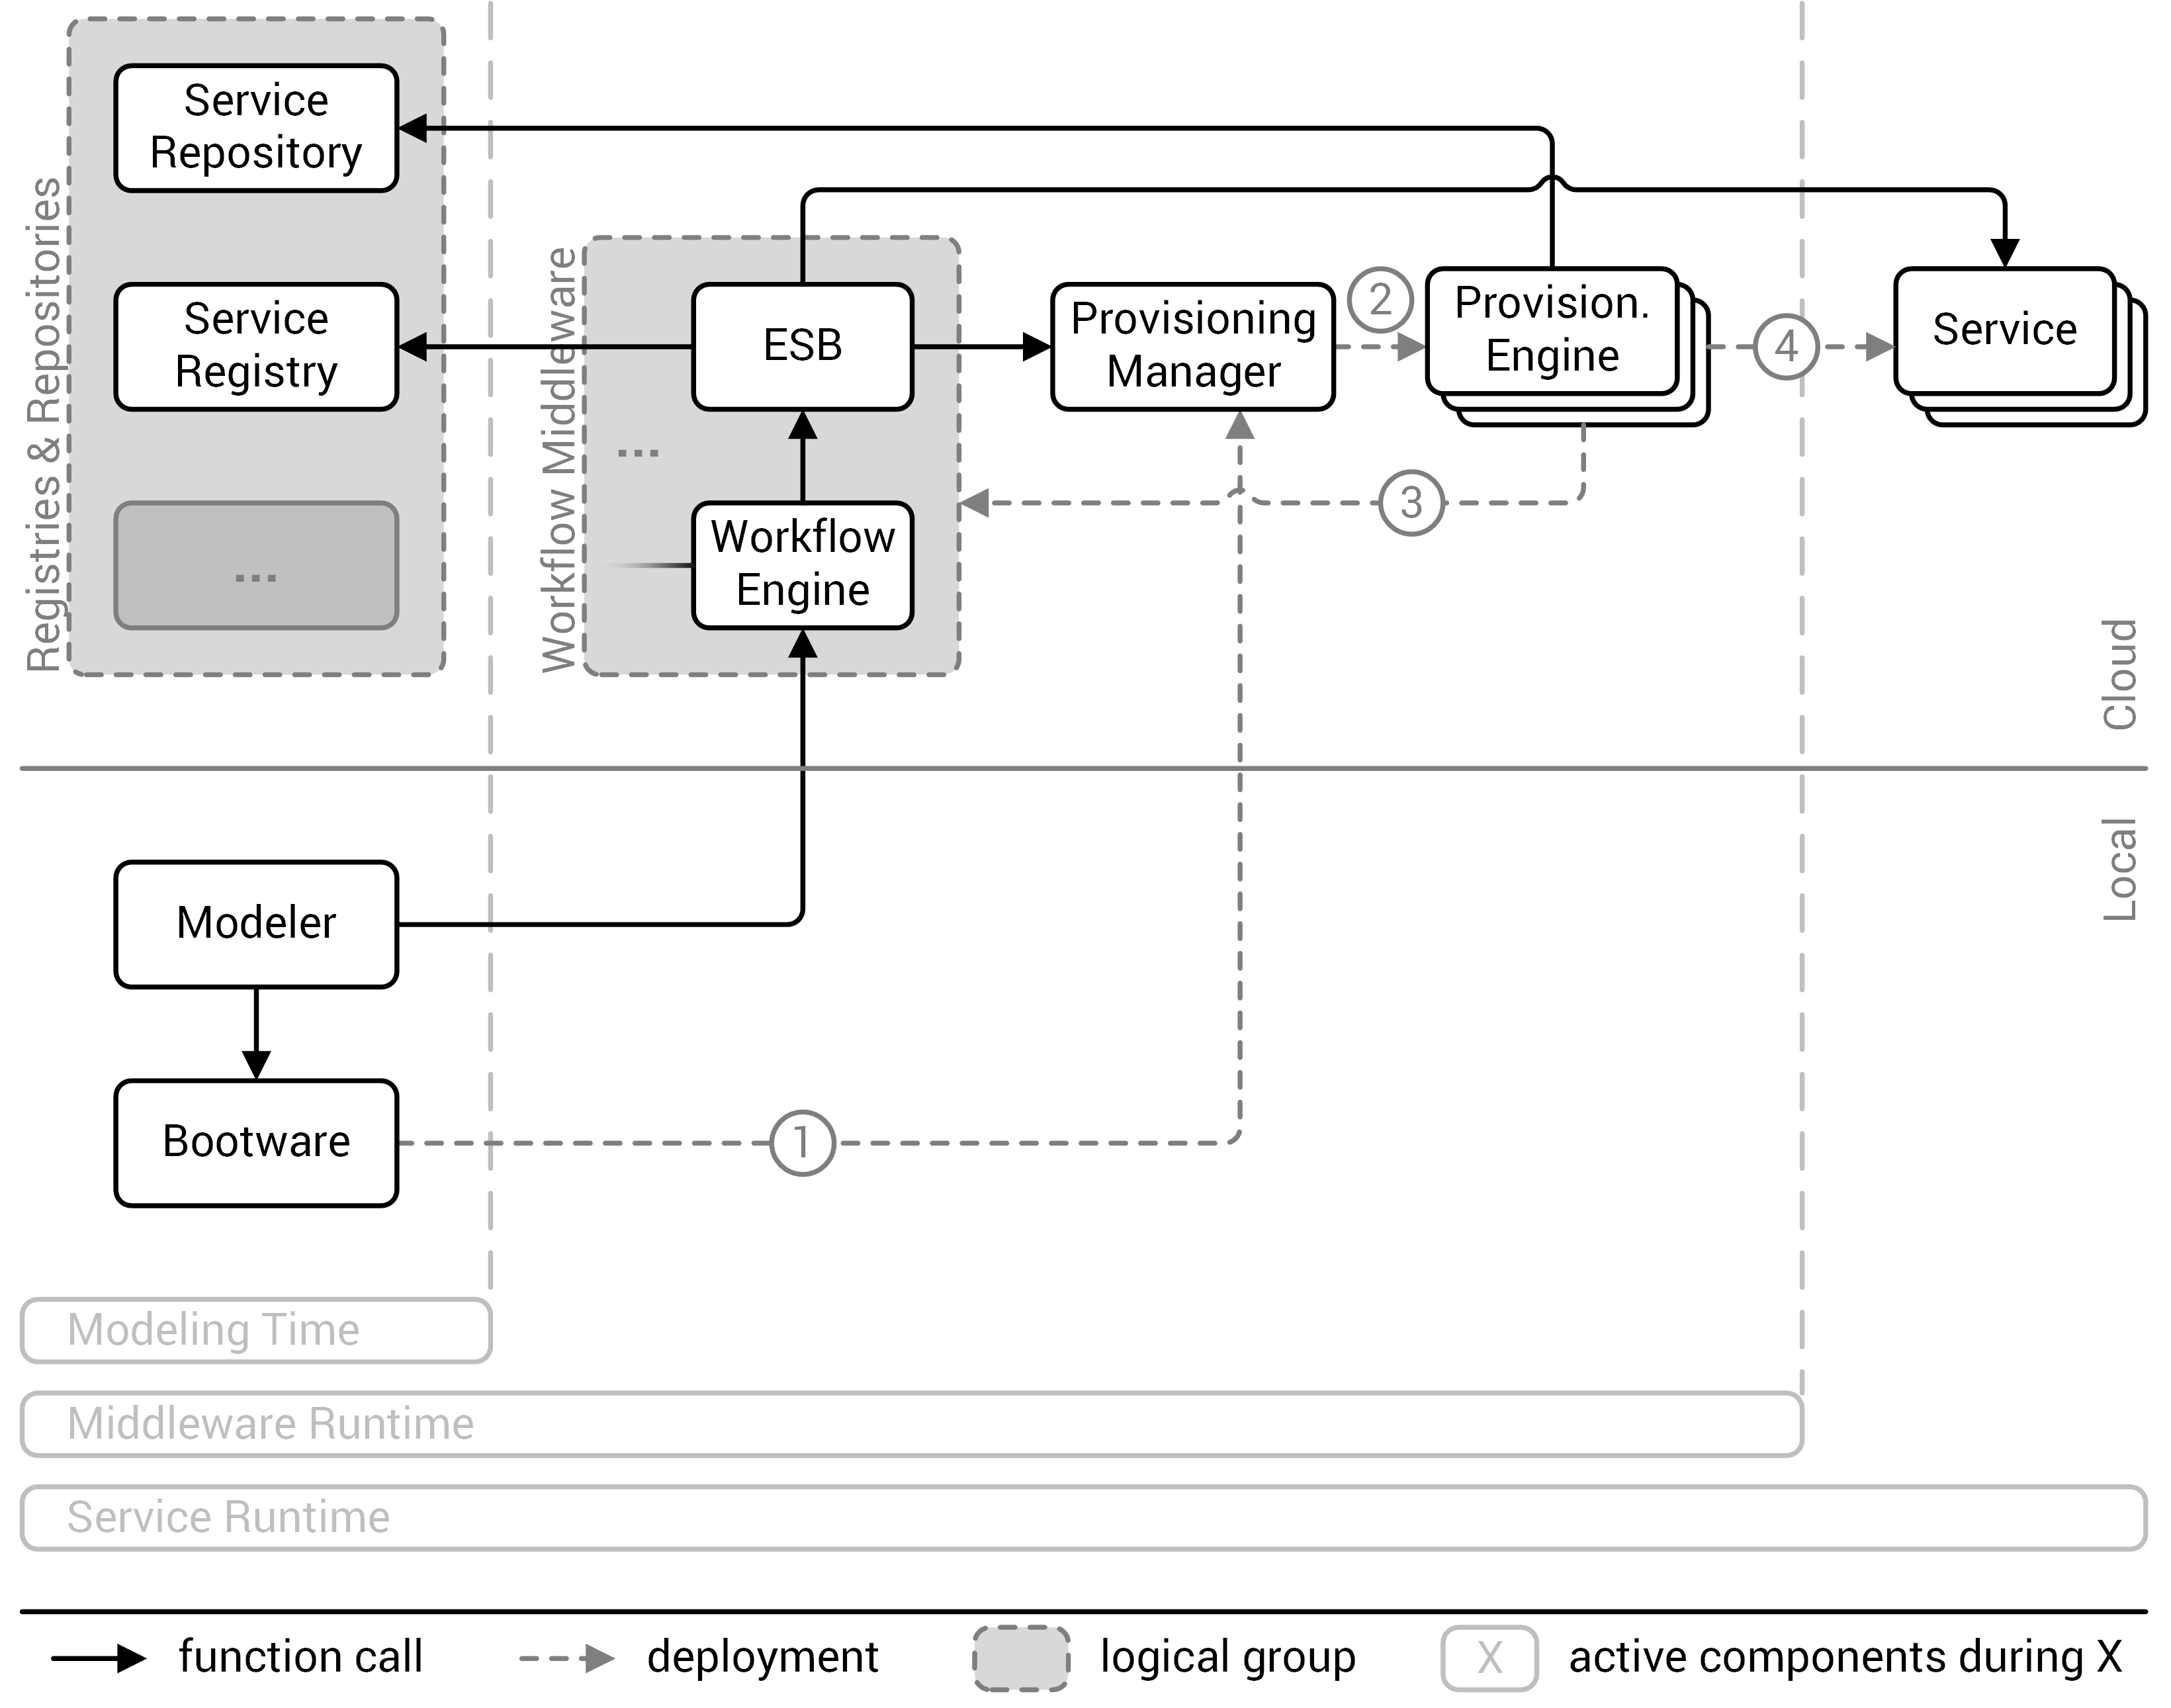
\includegraphics[resolution=600]{related/assets/valeri_architecture}
	\caption{Extended architecture with added provisioning manager}
	\label{image:valeri_architecture}
\end{figure}
